\documentclass[conference]{IEEEtran}
\IEEEoverridecommandlockouts
% The preceding line is only needed to identify funding in the first footnote. If that is unneeded, please comment it out.
\usepackage{cite}
\usepackage{amsmath,amssymb,amsfonts}
\usepackage{algorithmic}
\usepackage{graphicx}
\usepackage{textcomp}
\usepackage{xcolor}
\def\BibTeX{{\rm B\kern-.05em{\sc i\kern-.025em b}\kern-.08em
    T\kern-.1667em\lower.7ex\hbox{E}\kern-.125emX}}
\graphicspath{{Figures/}}

\begin{document}

\title{Secure Industrial Control System with Intrusion Detection\\
% {\footnotesize \textsuperscript{*}Note: Sub-titles are not captured in Xplore and
% should not be used}
}

\author{\IEEEauthorblockN{1\textsuperscript{st} Given Name Surname}
\IEEEauthorblockA{\textit{dept. name of organization (of Aff.)} \\
\textit{name of organization (of Aff.)}\\
City, Country \\
email address}
\and
\IEEEauthorblockN{Denis Ulybyshev}
\IEEEauthorblockA{\textit{Computer Science Department, CEROC} \\
\textit{Tennessee Technological University}\\
Cookeville, TN, United States of America \\
dulybyshev@tntech.edu}
\and
\IEEEauthorblockN{3\textsuperscript{rd} Given Name Surname}
\IEEEauthorblockA{\textit{dept. name of organization (of Aff.)} \\
\textit{name of organization (of Aff.)}\\
City, Country \\
email address}
\and
\IEEEauthorblockN{4\textsuperscript{th} Given Name Surname}
\IEEEauthorblockA{\textit{dept. name of organization (of Aff.)} \\
\textit{name of organization (of Aff.)}\\
City, Country \\
email address}
\and
\IEEEauthorblockN{5\textsuperscript{th} Given Name Surname}
\IEEEauthorblockA{\textit{dept. name of organization (of Aff.)} \\
\textit{name of organization (of Aff.)}\\
City, Country \\
email address}
\and
\IEEEauthorblockN{6\textsuperscript{th} Given Name Surname}
\IEEEauthorblockA{\textit{dept. name of organization (of Aff.)} \\
\textit{name of organization (of Aff.)}\\
City, Country \\
email address}
}

\maketitle

\begin{abstract}

\end{abstract}

\begin{IEEEkeywords}

\end{IEEEkeywords}

\section{Introduction}


\section{Related Work}


\section{Security in ICS}
\begin{figure}[htbp]
\centering
\centerline{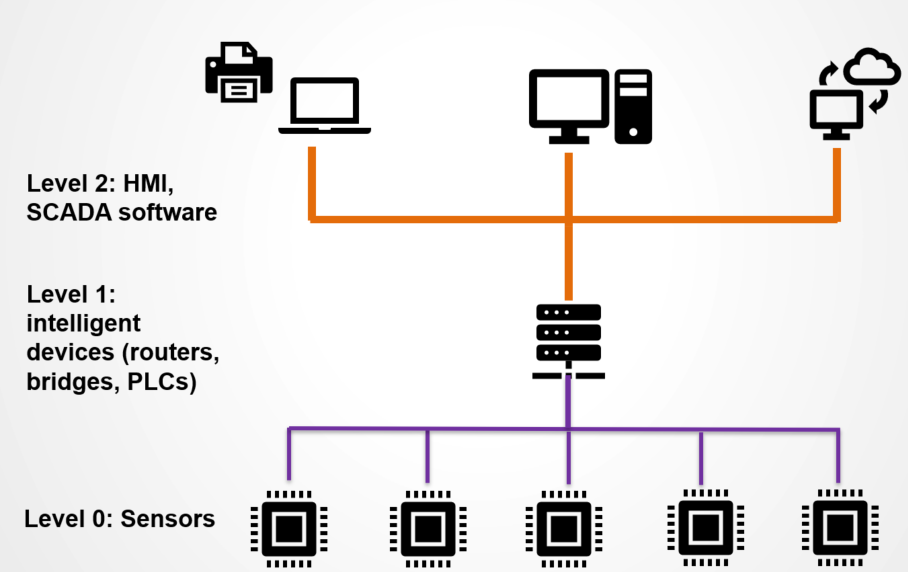
\includegraphics [width=9cm] {Architecture1.png}}
\caption{Industrial Control System Architecture}
\label{fig}
\end{figure}


\subsection{Software Solutions}\label{AA}
.

\subsection{Observed Gap}

\section{Proposed Architecture}

\section{Work in Progress and Future Direction}

\section{Conclusion}




\begin{thebibliography}{00}

\end{thebibliography}
\vspace{12pt}
\end{document}
